\chapter{Phương pháp kiểm chứng và môi trường UVM}
\label{ch:verification}

Chương này trình bày phương pháp xây dựng môi trường kiểm chứng cho thiết kế RTL ở
\cref{ch:architecture} theo các yêu cầu tại \cref{sec:req}: từ mục tiêu và chiến lược, kiến
trúc môi trường UVM, các cơ chế kiểm tra (\texttt{i3c\_scoreboard}, SVA, \FunctionalCoverage{}), đến
cách xây dựng kịch bản kiểm chứng.

\section{Mục tiêu và phạm vi kiểm chứng}
\label{sec:ver-scope}

Mục tiêu trong chương này hướng tới xác nhận thiết kế RTL ở \cref{ch:architecture} đáp ứng
toàn bộ yêu cầu chức năng tại \cref{sec:req}. Phạm vi được tổ chức bám sát hai interface
mà \Controller{} dùng để giao tiếp với bên ngoài: \gls{csr}/\gls{fifo} và bus SCL/SDA.

Phía \gls{csr}/\gls{fifo} là nơi \Host{} điều khiển \Controller{}. Tại đây, \Testbench{} kiểm tra các đường
truy cập vào \gls{csr}, \gls{dat}, \CommandResponseFifo{} và \TxRxFifo{} --- tức toàn bộ cơ chế nạp lệnh,
cấp dữ liệu và thu kết quả.

Phía bus SCL/SDA là nơi \Controller{} thực thi giao thức. Các kịch bản chính gồm I3C
\PrivateTransfer{} trong \gls{sdr} Mode, \ImmediateDataTransfer{}, CCC, \gls{entdaa} và
\iic{} Fast Mode. Ngoài các luồng bình thường, phạm vi bao gồm các tình huống lỗi: mỗi tình huống được dựng để kích
hoạt một mã lỗi mà thiết kế thực sự hiện thực (\cref{tab:err-status}), qua
đó kiểm chứng cơ chế báo lỗi và hủy giao dịch mô tả ở \cref{sec:arch-err}.

Các tính năng ngoài phạm vi tại \cref{tab:req-oos}, tiêu biểu là \gls{ibi} và \gls{hdr}, không được đặt
làm mục tiêu coverage vì RTL chưa hiện thực chúng. Nhờ đó, kết quả coverage không bị pha loãng bởi
những mục tiêu ngoài thiết kế.

\section{Chiến lược kiểm chứng}
\label{sec:ver-strategy}

Chiến lược kết hợp hai loại stimulus:
\begin{itemize}
	\item \textbf{Directed stimulus}: dùng kịch bản cố định cho những tình huống cần điều khiển
	      chính xác trình tự thao tác, dữ liệu vào và phản hồi của \Target{}.
	\item \textbf{Constrained-random stimulus}: mở rộng không gian kiểm chứng trong phạm vi hợp
	      lệ --- địa chỉ, độ dài và nội dung TX/RX data, cùng cách \Target{} phản hồi trên bus.
\end{itemize}

Mỗi \VirtualSequence{} được thiết kế quanh một mục tiêu kiểm chứng cụ thể. Randomization chỉ
thay đổi dữ liệu và điều kiện bên trong kịch bản, không thay thế tiêu chí pass/fail. Nhờ đó,
khi test thất bại, nguyên nhân vẫn truy được về một chức năng hoặc một tình huống giao thức
cụ thể.

Ba cơ chế kiểm tra được sử dụng song song:
\begin{itemize}
	\item Scoreboard: đối chiếu \CommandDescriptor{} và dữ liệu ghi vào \gls{csr}/\gls{fifo}
	      với giao dịch quan sát trên bus và \ResponseDescriptor{} do RTL trả về.
	\item SVA: mô tả và kiểm tra các điều kiện mà RTL phải thỏa mãn trong một hoặc
	      nhiều chu kỳ clock, như handshake ready/valid, hành vi của tín hiệu reset ngoài, trạng
	      thái \gls{fifo}, chuyển tiếp \gls{fsm} và yêu cầu hủy giao dịch.
	\item \FunctionalCoverage{}: ghi nhận các tình huống đã được kích hoạt, đặc biệt là các tổ
	      hợp giữa loại giao dịch, phản hồi của \Target{} và mã lỗi.
\end{itemize}

Cách phân vai này giúp kết quả không phụ thuộc một cơ chế duy nhất: \texttt{i3c\_scoreboard} và SVA kiểm
tra tính đúng đắn ở hai mức khác nhau, còn \FunctionalCoverage{} cho biết độ bao phủ các yêu cầu F1--F10.

\section{Kiến trúc tổng thể của \Testbench{}}
\label{sec:ver-arch}

Module \texttt{tb\_i3c\_top} là top-level của \Testbench{}. Module này tạo clock và tín hiệu reset ngoài, khởi
tạo \gls{dut} và hai SystemVerilog interface \texttt{reg\_if}, \texttt{i3c\_if}. Các virtual
interface được truyền vào những UVM component cần truy cập giao diện thông qua UVM
Configuration Database. \texttt{reg\_if} nối với giao diện CSR/FIFO, còn \texttt{i3c\_if} nối
với bus SCL/SDA và được \texttt{i3c\_agent} sử dụng để phản hồi giao dịch trên bus.

Bus SCL/SDA được mô hình hóa bằng \texttt{wire} có \texttt{pullup(weak1)} để phản ánh đặc tính
\OpenDrain{}. Ở pha \OpenDrain{}, DUT và \texttt{i3c\_agent} chỉ chủ động kéo bus xuống mức thấp,
còn mức cao được tạo khi bus được thả. Riêng với SDA, \Testbench{} dùng trạng thái
\OpenDrain{}/\PushPull{} do DUT cung cấp: thả hoặc kéo xuống ở pha \OpenDrain{} và lái cả hai
mức logic ở pha \PushPull{}.

Ở lớp UVM, \texttt{i3c\_base\_test} tạo \texttt{i3c\_env}, thiết lập cấu hình và chạy
\VirtualSequence{} được chọn khi mô phỏng. \texttt{i3c\_env} chứa các component:
\texttt{reg\_agent}, \texttt{i3c\_agent}, \texttt{i3c\_virtual\_sequencer},
\texttt{i3c\_scoreboard} và các coverage component.

Các monitor hoạt động độc lập với driver và không tự kết luận pass/fail. Chúng chuyển hoạt động
quan sát được trên giao diện thành item và phát qua \TLMAnalysisPort{}:
\begin{itemize}
	\item \texttt{reg\_monitor} đảm nhiệm phía CSR/FIFO.
	\item \texttt{i3c\_monitor} đảm nhiệm phía bus SCL/SDA.
	\item \texttt{i3c\_scoreboard} và các coverage component đăng ký nhận các item này.
\end{itemize}
Cơ chế mô hình tham chiếu tạo giá trị dự kiến và đối chiếu được trình bày tại
\cref{sec:ver-tlm}, còn thu thập \FunctionalCoverage{} tại \cref{sec:ver-cov}.

\begin{figure}[!htbp]
	\centering
	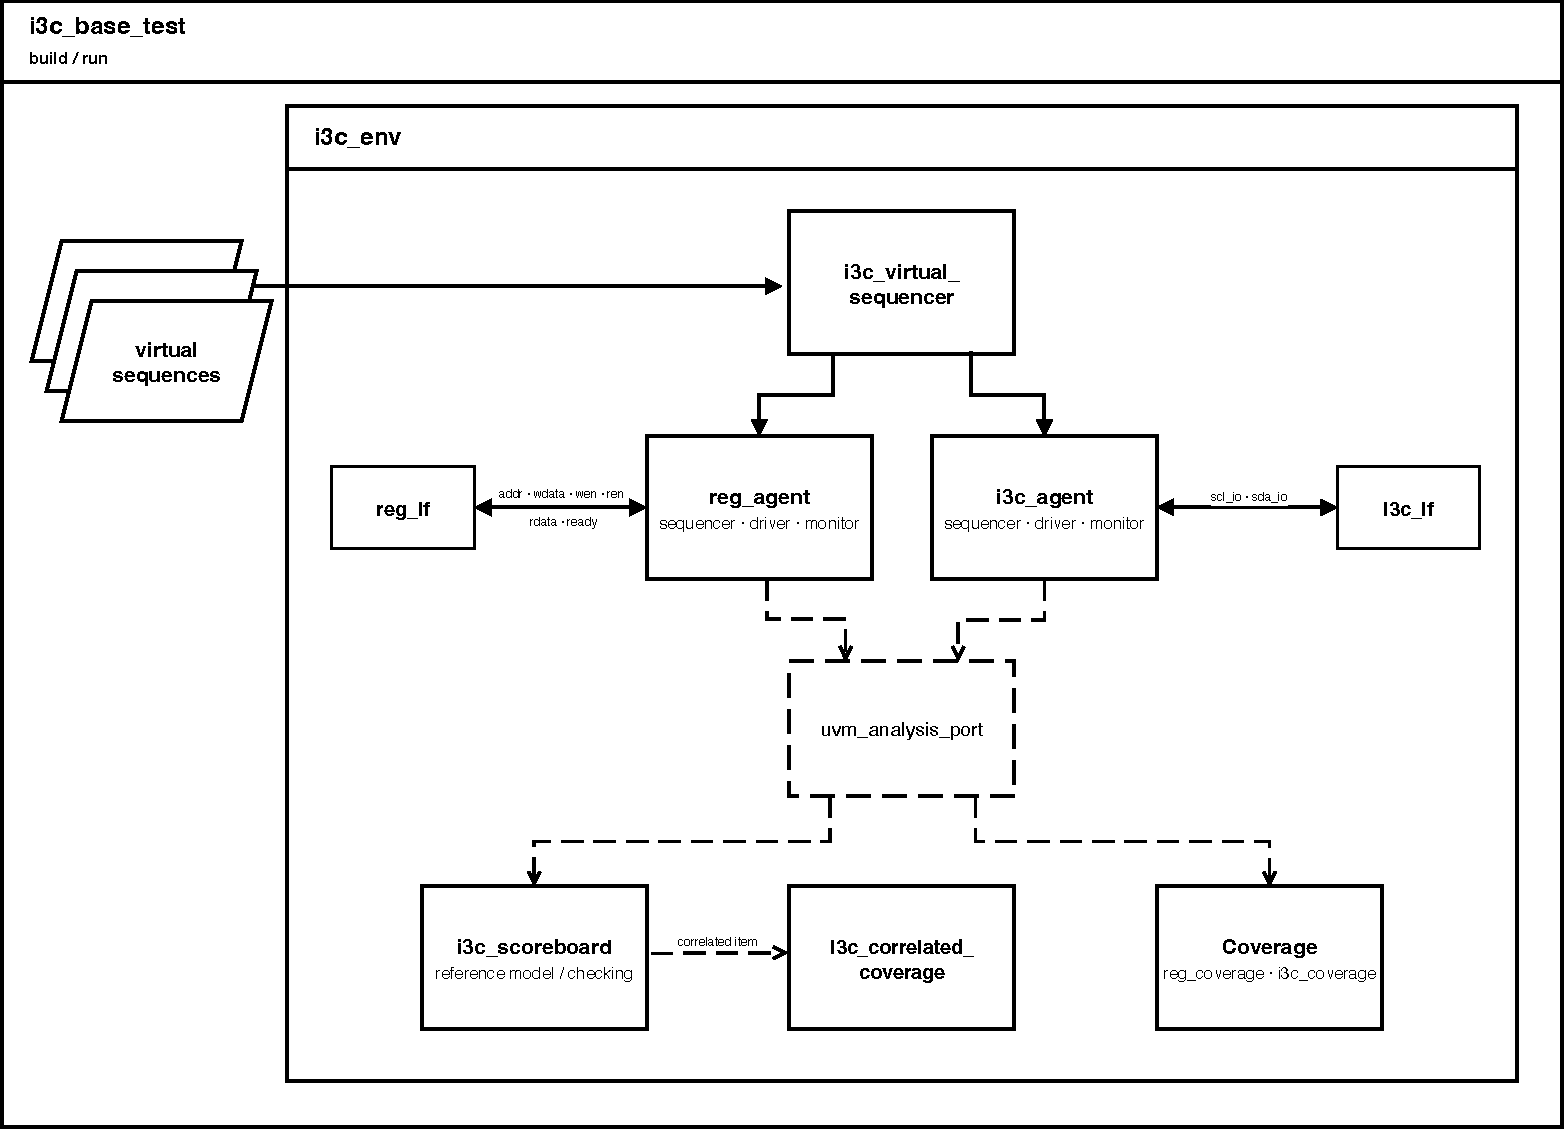
\includegraphics[max width=\textwidth, max totalheight=0.68\textheight]{figures/uvm_i3c_verification_architecture_uvm.pdf}
	\par\vspace{0.45em}
	\begin{tikzpicture}[
			legend text/.style={font=\footnotesize, anchor=west},
			control flow/.style={line width=0.8pt, -{Stealth[length=2.2mm,width=1.5mm]}},
			analysis flow/.style={line width=0.7pt, dashed, dash pattern=on 4pt off 2.5pt,
						-{Stealth[open,length=2.2mm,width=1.5mm]}}
		]
		\draw[control flow] (0,0) -- (1.10,0);
		\node[legend text, right=2mm] (control-label) at (1.10,0)
		{Control / direct interface flow};
		\coordinate (analysis-start) at ([xshift=9mm]control-label.east);
		\draw[analysis flow] (analysis-start) -- ++(1.10,0)
		coordinate (analysis-end);
		\node[legend text, right=2mm] at (analysis-end) {UVM TLM analysis transaction flow};
	\end{tikzpicture}
	\caption{Kiến trúc tổng thể của môi trường kiểm chứng I3C.}
	\label{fig:tb-arch}
\end{figure}

\section{Cơ chế \texttt{i3c\_scoreboard}}
\label{sec:ver-tlm}

\texttt{i3c\_scoreboard} nhận item từ \texttt{reg\_monitor} và \texttt{i3c\_monitor} qua \TLMAnalysisPort{}. Các item
phía \gls{csr}/\gls{fifo} được đưa vào mô hình tham chiếu (\ReferenceModel{}) để tạo giá trị dự kiến theo đặc tả. Các item phía bus, cùng dữ liệu đọc từ
\RxFifo{} và \ResponseFifo{}, được dùng làm dữ liệu thực tế để đối chiếu với giá trị dự kiến.

Mô hình tham chiếu trong \texttt{i3c\_scoreboard} lưu các thông tin cần dùng để kiểm tra giao
dịch hiện tại: bản sao \gls{dat}, \CommandDescriptor{}, TX data trong \TxFifo{}, RX data dự kiến
trong \RxFifo{} và \ResponseDescriptor{} dự kiến.
Từ phía \gls{csr}/\gls{fifo}, hai lần ghi vào
\CommandFifo{} được ghép thành \CommandDescriptor{} \CommandDescriptorWidth{}-bit rồi
mô hình tham chiếu giải mã các field \texttt{attr}, \texttt{tid}, \texttt{cmd}, \texttt{cp},
\texttt{dev\_idx}, \texttt{mode}, \texttt{rnw}, \texttt{wroc}, \texttt{toc} và
\texttt{data\_length} (\cref{app:desc}). Các thao tác ghi \gls{dat} được dùng để cập nhật bản sao
\gls{dat}. Dữ liệu ghi vào \TxFifo{} được dùng làm TX data dự kiến cho giao dịch ghi.

Khi nhận item từ \texttt{i3c\_monitor}, \texttt{i3c\_scoreboard} lấy giá trị dự kiến tương ứng
từ mô hình tham chiếu và kiểm tra theo loại giao dịch:
\begin{itemize}
	\item \textbf{Giao dịch ghi/đọc dữ liệu} (I3C \PrivateTransfer{}, \iic{} và
	      \ImmediateDataTransfer{}): đối chiếu \AddressHeader{}, \texttt{rnw}, TX/RX data và
	      ACK/NACK. Với pha dữ liệu \PushPull{} của I3C \gls{sdr} Mode, kiểm tra thêm \TBit{}, còn với
	      \ImmediateDataTransfer{}, TX data được lấy trực tiếp từ \CommandDescriptor{}.
	\item \textbf{CCC}: kiểm tra opcode, dạng Broadcast/Direct, địa chỉ \Target{} và
	      \EventsByte{}.
	\item \textbf{ENTDAA}: kiểm tra \gls{pid}/\gls{bcr}/\gls{dcr} của \Target{}, \DynamicAddress{} được
	      cấp, trường hợp \Target{} từ chối địa chỉ và RX data ghi về \RxFifo{}.
\end{itemize}
Sau khi giao dịch kết thúc,
\ResponseDescriptor{} do \Host{} đọc từ \ResponseFifo{} được so với các field
\texttt{err}, \texttt{tid} và \texttt{data\_length} (\cref{app:desc}).

\section{Kiểm tra bằng SVA}
\label{sec:ver-sva}

SVA kiểm tra các thuộc tính cục bộ theo thời gian mà \texttt{i3c\_scoreboard} khó bao quát, đồng
thời báo lỗi ngay tại chu kỳ vi phạm, gồm handshake ready/valid, chuyển tiếp \gls{fsm}, bộ đếm,
quy tắc lái SDA (\OpenDrain{}/\PushPull{}, tránh tranh chấp) và chiếm quyền SDA khi takeover, đối
chiếu đồng thời tín hiệu DUT với net của mô hình chân I/O.

Mỗi assertion mang label \texttt{ap\_*}. Trừ các bất biến luôn đúng (kể cả khi idle hoặc tín hiệu reset ngoài được kích hoạt), mỗi
assertion có một cover property \texttt{cp\_*} tương ứng để phân biệt pass thực sự với vacuous
pass. Bằng chứng kiểm chứng dựa trên kết quả kích hoạt và pass/miss, không dựa trên số lượng
property (\cref{ch:results}).

\Cref{lst:ver-sva-tbit} minh họa property \TBit{} của I3C \PrivateWrite{}
. Ở pha dữ liệu \PushPull{}, mỗi byte kết thúc bằng \TBit{}
mang odd parity. Khi \gls{fsm} đến thời điểm phát \TBit{}, assertion yêu cầu DUT phát đúng một bit
với giá trị parity tương ứng.

\begin{lstlisting}[language=Verilog,caption={SVA kiểm tra T-Bit odd parity của I3C \PrivateWrite{}.},label={lst:ver-sva-tbit}]
// SDR Private Write data phase: T-Bit must carry odd parity
ap_sdr_write_tbit_parity:
  assert property (@(posedge clk_i) disable iff (!rst_ni)
    state_q == IssueI3CWrite && sdr_regular_i3c_write() &&
    remaining_len_q > 16'h0 &&
    issue_phase_q > PhaseAddrAck && !issue_phase_q[0]
    |->
    bus_tx_req_bit && !bus_tx_req_byte &&
    bus_tx_req_value === {7'b0, ~^current_tx_byte});

cp_sdr_write_tbit_parity:
  cover property (@(posedge clk_i) disable iff (!rst_ni)
    state_q == IssueI3CWrite && sdr_regular_i3c_write() &&
    remaining_len_q > 16'h0 &&
    issue_phase_q > PhaseAddrAck && !issue_phase_q[0] &&
    bus_tx_req_bit && !bus_tx_req_byte &&
    bus_tx_req_value === {7'b0, ~^current_tx_byte});
\end{lstlisting}

\section{Chiến lược \FunctionalCoverage{}}
\label{sec:ver-cov}

\FunctionalCoverage{} được tổ chức thành ba lớp tương ứng ba nguồn quan sát:
\begin{itemize}
	\item \texttt{reg\_coverage}: bao phủ DAT \texttt{device}, các field của
	      \CommandDescriptor{}, chính sách điều khiển \Host{} và thao tác phần mềm trên các queue port.
	\item \texttt{i3c\_coverage}: bao phủ các pha địa chỉ và giao dịch đã tái tạo trên bus --- giao
	      thức I3C/\iic{}, chiều đọc/ghi, số byte dữ liệu, ACK/NACK, START/repeated START, CCC và từng vòng ENTDAA.
	\item \texttt{i3c\_correlated\_coverage}: bao phủ các quan hệ xuyên suốt chỉ xác định được
	      sau khi \texttt{i3c\_scoreboard} đã ghép các field của \CommandDescriptor{}, kết quả bus và
	      các field \texttt{err}/\texttt{data\_length} của \ResponseDescriptor{}; trong đó có
	      \TBit{}, toàn vẹn dữ liệu và giao dịch dừng giữa chừng.
\end{itemize}

Các bin được thiết kế quanh những tình huống then chốt của F1--F10 (\cref{tab:req-func}) và được
chia hai vai. Nhóm \emph{closure bin} là mục tiêu bắt buộc phải kích hoạt: mọi loại giao dịch
trong phạm vi phải xuất hiện ít nhất một lần, mỗi \texttt{err} phải xuất hiện đúng với
\texttt{attr} sinh ra nó qua cross \texttt{err} $\times$ \texttt{attr}, cùng các tình huống biên được nhắm riêng như
độ dài TX/RX data tại biên \gls{dword}, \Target{} từ chối \DynamicAddress{} trong \gls{entdaa}, ACK/NACK và
\TBit{} trên bus (chi tiết ánh xạ từng yêu cầu sang cơ chế coverage tương ứng xem
\cref{tab:req-ver-map}).

Các bin còn lại chỉ mang tính \emph{diagnostic}, dùng để quan sát và không được cộng vào tổng số
bin dùng tính tỷ lệ closure. Coverpoint thành phần của một cross đã đóng vai closure owner cũng
được xếp làm diagnostic để tránh cộng trùng. Illegal bin chỉ dùng cho tình huống giao thức thực
sự cấm. Tính năng ngoài phạm vi không bị đánh dấu illegal chỉ vì RTL không hỗ trợ.

Về hiện thực, mỗi lớp là một \texttt{uvm\_subscriber}. Ba lớp lần lượt nhận item qua
\TLMAnalysisPort{} của \texttt{reg\_monitor}, \texttt{i3c\_monitor} và
\texttt{i3c\_scoreboard}. Covergroup được sample theo sự kiện giao dịch chứ không theo clock:
một mẫu chỉ được ghi khi một truy cập thanh ghi, một giao dịch bus hoặc một item đã ghép đủ
context thực sự hoàn tất.

Để thể hiện trực quan phạm vi của từng lớp, \cref{tab:functional-cov-matrix} chuyển các
covergroup thành ma trận phân bổ theo nhóm chức năng. Ký hiệu C chỉ các bin trực tiếp tham gia
closure, D chỉ các coverpoint thành phần được giữ để chẩn đoán, còn C/D cho biết nhóm vừa có
cross sở hữu closure vừa có các coverpoint chẩn đoán. Dấu ``--'' nghĩa là hạng mục không được
sample tại lớp quan sát tương ứng; nó không mang nghĩa chưa được kiểm chứng. Cách biểu diễn này
giữ nguyên nguyên tắc một hành vi chỉ có một coverage owner, thay vì tạo lại cùng một cross ở
nhiều subscriber.

\begin{table}[!htbp]
	\centering
	\caption{Ma trận phân bổ Functional Coverage theo lớp quan sát.}
	\label{tab:functional-cov-matrix}
	\footnotesize
	\setlength{\tabcolsep}{3pt}
	\renewcommand{\arraystretch}{1.08}
	\begin{tabular}{C{1.55cm} L{6.15cm} C{1.35cm} C{1.35cm} C{1.55cm}}
		\toprule
		\multirow{2}{*}{\textbf{Nhóm}}                                                & \multirow{2}{*}{\textbf{Không gian tình huống được sample}}
		                                                                              & \multicolumn{3}{c}{\textbf{Lớp quan sát}}                                                                                                           \\
		\cmidrule(lr){3-5}
		                                                                              &                                                                                                & \rotatebox{90}{\texttt{reg\_coverage}}
		                                                                              & \rotatebox{90}{\texttt{i3c\_coverage}}
		                                                                              & \rotatebox{90}{\texttt{correlated\_coverage}}                                                                                                       \\
		\midrule
		\multirow{3}{*}{\shortstack{Ý định\\phía \Host{}}}
		                                                                              & DAT \texttt{device}                                                                            & C                                      & --  & --  \\
		                                                                              & \texttt{attr}, \texttt{rnw}, \texttt{toc}, \texttt{wroc},
		\texttt{data\_length}/\texttt{dtt}, \texttt{dev\_idx}, \texttt{mode},
		\texttt{cp}, \texttt{cmd} và \texttt{sre}                                     & C/D                                                                                            & --                                     & --        \\
		                                                                              & \texttt{attr} $\times$ DAT \texttt{device}; \texttt{bus\_enable},
		\texttt{broadcast\_enable}, \texttt{hc\_abort} và \texttt{queue\_op}
		                                                                              & C/D                                                                                            & --                                     & --        \\
		\midrule
		\multirow{5}{*}{\shortstack{Quan sát\\trên bus}}
		                                                                              & \texttt{addr\_class} $\times$ \texttt{addr\_nack}; \texttt{start\_source}                      & --                                     & C/D & --  \\
		                                                                              & \texttt{i3c} $\times$ \texttt{bus\_op} $\times$ \texttt{num\_data};
		\texttt{trailing\_bytes}
		                                                                              & --                                                                                             & C/D                                    & --        \\
		                                                                              & \texttt{previous\_op} $\times$ \texttt{current\_op}
		                                                                              & --                                                                                             & C/D                                    & --        \\
		                                                                              & \texttt{i3c\_direct} $\times$ \texttt{CCC} $\times$ \texttt{addr\_nack}                        & --                                     & C/D & --  \\
		                                                                              & \texttt{daa\_round\_outcome}; \texttt{daa\_assigned\_addr\_class}                              & --                                     & C   & --  \\
		\midrule
		\multirow{7}{*}{\shortstack{Tương\\quan\\đầu cuối}}
		                                                                              & \texttt{attr=ImmediateDataTransfer}: \texttt{target\_is\_i3c} $\times$
		\texttt{dtt}; \texttt{nack\_phase}
		                                                                              & --                                                                                             & --                                     & C/D       \\
		                                                                              & \texttt{attr} $\times$ \texttt{err}; \texttt{data\_length} và \texttt{response\_len\_relation}
		                                                                              & --                                                                                             & --                                     & C/D       \\
		                                                                              & \texttt{daa\_result}, \texttt{err}, \texttt{dev\_idx} và \texttt{dev\_count}                   & --                                     & --  & C/D \\
		                                                                              & \texttt{preamble\_policy}; \texttt{response\_addr\_phase} $\times$
		\texttt{address\_acked} $\times$ \texttt{err}                                 & --                                                                                             & --                                     & C/D       \\
		                                                                              & \texttt{attr} $\times$ \texttt{wroc} $\times$ \texttt{err} $\times$ \texttt{response\_present}
		                                                                              & --                                                                                             & --                                     & C/D       \\
		                                                                              & \texttt{final\_t\_bit} $\times$ \texttt{length\_outcome};
		\texttt{nack\_position}; \texttt{sre} $\times$ \texttt{short\_boundary}       & --                                                                                             & --                                     & C/D       \\
		                                                                              & \texttt{protocol\_direction}, \texttt{abort\_cause} $\times$ \texttt{abort\_point},
		\texttt{recovery\_source}, \texttt{command\_boundary} và \texttt{stall\_type} & --                                                                                             & --                                     & C/D       \\
		\bottomrule
	\end{tabular}
\end{table}

Ý nghĩa các coverpoint trong \cref{tab:functional-cov-matrix} không thuộc \CommandDescriptor{},
\ResponseDescriptor{} hay \gls{csr} được giải thích tại \cref{app:cov-legend}.

Tổng hợp lại, \cref{tab:req-ver-map} cho thấy ba cơ chế kiểm tra trên phối hợp phủ các yêu cầu
chức năng F1--F10 như thế nào. Đây cũng là khung đối chiếu khi đánh giá kết quả ở \cref{ch:results}.

\begin{table}[!htbp]
	\centering
	\caption{Ánh xạ yêu cầu sang cơ chế kiểm chứng chính.}
	\label{tab:req-ver-map}
	\begin{tabular}{C{2.0cm} L{10.5cm}}
		\toprule
		\textbf{Yêu cầu} & \textbf{Cơ chế và nội dung kiểm tra}                                                                                                                                                                                           \\
		\midrule
		F1--F3           & \texttt{i3c\_monitor} tái tạo giao dịch. \texttt{i3c\_scoreboard} đối chiếu \texttt{attr}, \texttt{rnw}, \texttt{data\_length} và dữ liệu. SVA kiểm tra \TBit{}. Coverage ghi nhận các giao dịch I3C SDR Mode.                 \\
		F4               & Driver lưu ngữ cảnh CCC. \texttt{i3c\_scoreboard} đối chiếu \texttt{cmd} và dạng Broadcast/Direct. Coverage ghi nhận các lệnh CCC.                                                                                             \\
		F5               & \texttt{i3c\_agent} tham gia ENTDAA. \texttt{i3c\_scoreboard} đối chiếu PID/BCR/DCR, \DynamicAddress{} và DAT/RX. SVA kiểm tra FSM. Coverage ghi nhận các kịch bản DAA.                                                        \\
		F6               & \texttt{i3c\_agent} tạo ACK/NACK và dữ liệu \iic{}. \texttt{i3c\_scoreboard} đối chiếu TX/RX. SVA kiểm tra bộ đếm và quy tắc lái bus.                                                                                          \\
		F7               & \texttt{reg\_monitor} và \texttt{i3c\_scoreboard} kiểm tra CSR/FIFO. SVA kiểm tra handshake và trạng thái FIFO. Coverage ghi nhận truy cập và cấu hình thanh ghi.                                                              \\
		F8               & Mô hình tham chiếu tạo \ResponseDescriptor{} dự kiến. \texttt{i3c\_scoreboard} đối chiếu \texttt{err}, \texttt{tid} và \texttt{data\_length}. \texttt{i3c\_correlated\_coverage} ghi nhận \texttt{err} $\times$ \texttt{attr}. \\
		F9               & \texttt{i3c\_scoreboard} theo dõi yêu cầu hủy giao dịch từ \Host{}. SVA kiểm tra việc hủy giao dịch, kết thúc ở pha hợp lệ và quy tắc lái bus SDA.                                                                             \\
		F10              & \texttt{reg\_monitor} đối chiếu CSR cấu hình các tham số thời gian. Monitor xác định chu kỳ SCL. Cover property định thời được kích hoạt cho các tình huống sau reset ngoài, ghi và đọc lại.                                   \\
		\bottomrule
	\end{tabular}
\end{table}

\section{\texttt{reg\_agent}}
\label{sec:ver-regagent}

\texttt{reg\_agent} đóng vai \Host{}, chủ động điều khiển giao diện CSR/FIFO của \Controller{}.
\texttt{reg\_driver} điều khiển \texttt{addr}, \texttt{wdata}, \texttt{wen}/\texttt{ren} rồi chờ
ready để thực hiện từng lần đọc hoặc ghi thanh ghi. \texttt{reg\_monitor} phát các truy cập đã hoàn
tất qua \TLMAnalysisPort{}.

Vì giao thức thanh ghi đơn giản, \texttt{reg\_driver} chỉ là một engine đọc/ghi đồng bộ theo handshake
ready/valid.
Lớp này cung cấp các thao tác đọc/ghi đơn cùng helper dựng \CommandDescriptor{}
\CommandDescriptorWidth{}-bit rồi phát thành hai lần ghi 32-bit. \VirtualSequence{} dùng chúng
để cấu hình \gls{dat}, nạp \TxFifo{}, ghi \CommandFifo{}, chờ \Controller{} hoàn tất giao dịch rồi
đọc \RxFifo{} và \ResponseFifo{}.
Nhờ \texttt{reg\_driver} độc lập với ngữ nghĩa giao dịch, cùng một Agent phục vụ cả test \gls{csr}
thuần túy lẫn các kịch bản giao dịch đầy đủ.

\section{\texttt{i3c\_agent}}
\label{sec:ver-i3cagent}

\texttt{i3c\_agent} đóng vai một \Target{} có thể lập trình trên bus. \texttt{i3c\_driver} phản hồi
\AddressHeader{}, phát ACK/NACK theo cấu hình, nhận TX data, phát RX data và tham
gia \gls{entdaa}. \texttt{i3c\_monitor} tái tạo giao dịch từ tín hiệu SDA/SCL độc lập với \texttt{i3c\_driver}, nên phát hiện
được cả sai lệch do chính \texttt{i3c\_driver} tạo ra.

\texttt{i3c\_driver} hoạt động theo một \gls{fsm} gồm \DriverPhaseCount{} trạng thái. Vai trò của từng
trạng thái được trình bày trong \cref{tab:drv-phase}. \gls{fsm} đồng bộ theo cạnh SCL và các event
trong interface, nên hành vi của Driver không phụ thuộc tần số SCL được cấu hình.

\begin{table}[!htbp]
	\centering
	\caption{Các trạng thái của FSM trong \texttt{i3c\_driver}.}
	\label{tab:drv-phase}
	\begin{tabular}{L{4.0cm} L{9.2cm}}
		\toprule
		\textbf{Trạng thái}       & \textbf{Chức năng}                                                                                  \\
		\midrule
		\texttt{DrvIdle}          & Chờ \Host{} phát START.                                                                             \\
		\texttt{DrvAddr}          & Lấy mẫu \AddressHeader{} trong pha \OpenDrain{}.                                                    \\
		\texttt{DrvAddrPushPull}  & Lấy mẫu địa chỉ trong pha \PushPull{} (sau \RepeatedSTART{}) và chọn ENTDAA, \DirectCCC{} hoặc ACK. \\
		\texttt{DrvAck}           & Phát ACK/NACK cho địa chỉ theo cấu hình \Target{}.                                                  \\
		\texttt{DrvSelectNext}    & Chọn nhánh đọc, ghi, CCC hoặc kết thúc giao dịch.                                                   \\
		\texttt{DrvWr}            & Nhận dữ liệu \iic{} và phản hồi ACK/NACK từng byte.                                                 \\
		\texttt{DrvWrPushPull}    & Nhận dữ liệu I3C cùng \TBit{} ở chế độ push-pull.                                                   \\
		\texttt{DrvRd}            & Phát dữ liệu \iic{} và lấy mẫu ACK/NACK từ \Host{}.                                                 \\
		\texttt{DrvRdPushPull}    & Phát dữ liệu I3C cùng \TBit{} ở chế độ push-pull.                                                   \\
		\texttt{DrvEntdaa}        & Phát PID/BCR/DCR, nhận và ACK/NACK \DynamicAddress{}.                                               \\
		\texttt{DrvStop}          & Nhả bus và chờ kết thúc phiên xử lý.                                                                \\
		\texttt{DrvBcastDispatch} & Nhận opcode và chọn Broadcast CCC, \DirectCCC{} hoặc ENTDAA.                                        \\
		\texttt{DrvCccData}       & Xử lý địa chỉ \Target{} và dữ liệu của CCC.                                                         \\
		\bottomrule
	\end{tabular}
\end{table}

\texttt{i3c\_device\_response\_seq} cấu hình Static/\DynamicAddress{}, RX data, điểm NACK, \TBit{}
và \gls{pid}/\gls{bcr}/\gls{dcr} cho một giao dịch, gửi xuống \texttt{i3c\_driver} dưới dạng một \texttt{i3c\_seq\_item}
mang sẵn đủ trường cho cả ba khả năng: tham gia ENTDAA, trả lời \DirectCCC{} hay thực hiện I3C \PrivateTransfer{}. Vì vậy \texttt{i3c\_driver} phải tự nhớ CCC nào vừa đi qua
mới biết dùng đúng nhóm trường nào trong cấu hình đó để tiếp tục điều khiển phản hồi --- tham gia
DAA, nhận \EventsByte{} hay thực hiện I3C \PrivateTransfer{}.

\section{\texttt{i3c\_virtual\_sequencer} và thư viện \VirtualSequence{}}
\label{sec:ver-vseq}

\VirtualSequence{} là đơn vị kịch bản của môi trường kiểm chứng. Mỗi kịch bản hoàn chỉnh cần
phối hợp hai phía: \Host{} nạp cấu hình và lệnh qua \gls{csr}/\gls{fifo}, còn trên bus một \Target{} phản
hồi đúng lúc trên SCL/SDA. \VirtualSequence{} điều phối hai phía đó trong một kịch bản, từ
chuẩn bị \gls{dat} và phát \CommandDescriptor{} cho tới chờ giao dịch kết thúc và đọc lại kết quả.

\begin{table}[!htbp]
	\centering
	\caption{Phân nhóm \VirtualSequence{} theo mục tiêu kiểm chứng.}
	\label{tab:vseq-cat}
	\begin{tabular}{L{3.0cm} C{1.6cm} L{8.5cm}}
		\toprule
		\textbf{Nhóm}                & \textbf{Số lượng}             & \textbf{Mục tiêu chính}                                                                                                                                                          \\
		\midrule
		Bus                          & \BusVseqCount{}               & Kiểm chứng lớp vật lý, START/\RepeatedSTART{}/STOP, định thời, tuần tự hóa dữ liệu và mô hình chân I/O.                                                                          \\
		CSR                          & \CsrVseqCount{}               & Kiểm chứng giá trị mặc định sau reset ngoài, DAT, ghép \CommandDescriptor{}, trạng thái và địa chỉ chưa ánh xạ.                                                                  \\
		FIFO                         & \FifoVseqCount{}              & Kiểm chứng thứ tự, trạng thái đầy/rỗng, đọc--ghi đồng thời, xóa và quay vòng con trỏ.                                                                                            \\
		SDR write                    & \SdrWriteVseqCount{}          & Kiểm chứng I3C \PrivateWrite{} với nhiều độ dài, giao dịch liên tiếp, DAT, \texttt{toc} và \texttt{Ovl}.                                                                         \\
		SDR read                     & \SdrReadVseqCount{}           & Kiểm chứng I3C \PrivateRead{} với nhiều độ dài, giao dịch liên tiếp, DAT, \texttt{toc}, \texttt{Ovl} và \texttt{I3cShortReadErr}.                                                \\
		\ImmediateDataTransfer{}     & \ImmediateVseqCount{}         & Kiểm chứng dữ liệu nhúng trong \CommandDescriptor{} với I3C/\iic{}, \texttt{dtt}, \texttt{toc} và NACK.                                                                          \\
		CCC                          & \CccVseqCount{}               & Kiểm chứng ENEC và DISEC ở dạng \BroadcastCCC{} và \DirectCCC{}.                                                                                                                 \\
		DAA                          & \DaaVseqCount{}               & Kiểm chứng ENTDAA với không, một hoặc nhiều \Target{}, biên DAT, \texttt{NACK} và \texttt{NotSupported}.                                                                         \\
		\iic{}                       & \IicVseqCount{}               & Kiểm chứng đọc/ghi \iic{}, độ dài dữ liệu, nhận một phần và \texttt{I2cDataNack}.                                                                                                \\
		\ResponseDescriptor{} và lỗi & \ResponseVseqCount{}          & Kiểm chứng các field \texttt{err}, \texttt{tid}, \texttt{data\_length}; các giá trị \texttt{Success}, \texttt{HcAborted}, \texttt{NotSupported}; hai loại reset và backpressure. \\
		\midrule
		\textbf{Tổng}                & \textbf{\RunnableVseqCount{}}                                                                                                                                                                                    \\
		\bottomrule
	\end{tabular}
\end{table}

Khả năng điều phối này đến từ \texttt{i3c\_virtual\_sequencer}. \texttt{i3c\_virtual\_sequencer} không sinh stimulus mà
chỉ giữ handle tới Sequencer của cả hai Agent: \texttt{reg\_agent} và \texttt{i3c\_agent}. Trong cùng
một \VirtualSequence{}, \texttt{i3c\_device\_response\_seq} của \Target{} được khởi động trên
\texttt{i3c\_sequencer} và chạy song song (\texttt{fork}) với các thao tác CSR/FIFO phát trên
\texttt{reg\_sequencer}. Vì vậy, hai Agent vẫn độc lập và tái sử dụng được, còn việc bắt nhịp giữa chúng được gói gọn bên
trong kịch bản.

Nguyên tắc xuyên suốt thư viện là mỗi \VirtualSequence{} định nghĩa một trường hợp kiểm chứng:
nó chỉ chịu trách nhiệm sinh stimulus cho kịch bản được định sẵn, còn việc đối chiếu đúng/sai được
giao cho \texttt{i3c\_scoreboard}. Cách phân vai này vừa tránh kiểm tra trùng lặp, vừa giúp khi một test thất
bại thì nguyên nhân truy được về đúng một cơ chế kiểm tra duy nhất.

\Testbench{} hiện triển khai \RunnableVseqCount{} \VirtualSequence{}, chia thành
\VseqCategoryCount{} nhóm như \cref{tab:vseq-cat}. Danh sách đầy đủ các kịch bản trong từng
nhóm được liệt kê ở \cref{app:regression}.

\section{Tổng kết chương}
\label{sec:ver-summary}

Môi trường kết hợp \texttt{reg\_agent} và \texttt{i3c\_agent} dưới một \texttt{i3c\_virtual\_sequencer}, dùng
\texttt{i3c\_scoreboard} để đối chiếu tính đúng đắn ở mức giao dịch, SVA cho thuộc tính cục bộ và \FunctionalCoverage{}
ba lớp để xác định độ bao phủ. Cấu trúc này bao phủ cả register interface phía phần mềm lẫn hành
vi giao thức mà không đặt logic kiểm tra trong \VirtualSequence{}. Kết quả áp dụng môi trường
này --- pass/fail, coverage và SVA --- được trình bày tại \cref{ch:results}.
